\tikzset{>=latex} % for LaTeX arrow head

% DRAW PLOT: sin, cos, tan





% AXIS ENVIRONMENT: arcsin, arccos, arctan


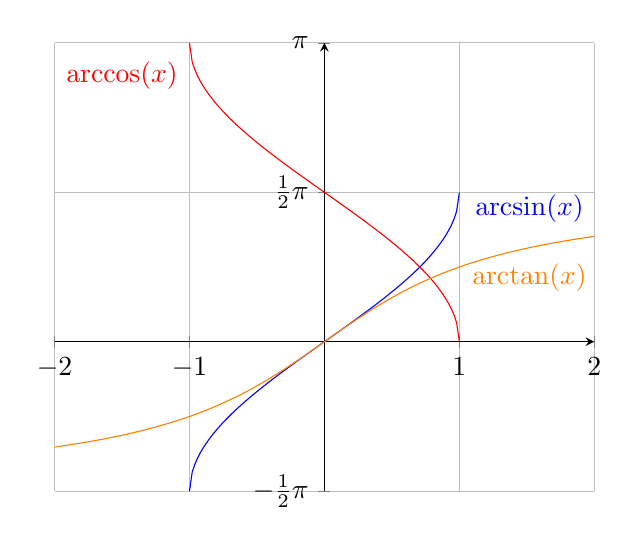
\begin{tikzpicture}
\begin{axis}[enlargelimits=false,
             axis lines=middle,
             xtick={-2,-1,0,1,2},
             ytick={-1.570780, 1.570780, 3.14159},
             yticklabels={$-\frac{1}{2}\pi$,$\frac{1}{2}\pi$,$\pi$},
             grid=major,
             samples=100
             ]
  
  % arcsin
  \addplot[domain=-1:1,no marks,blue] {rad(asin(x))};
  \node at (axis cs:1.52,1.4){\color{blue}$\arcsin(x)$};
  
  % arccos
  \addplot[domain=-1:1,no marks,red] {rad(acos(x))};
  \node at (axis cs:-1.5,2.8){\color{red}$\arccos(x)$};
  
  % arctan
  \addplot[domain=-2:2,no marks,orange] {rad(atan(x))};
  \node at (axis cs:1.52,.67){\color{orange}$\arctan(x)$};
  
\end{axis}
\end{tikzpicture}
